\chapter{Light Cones, Geodesics, and the Schwarzschild Horizon}

We begin exactly where this lecture begins: by stepping back to special relativity and rebuilding the causal vocabulary before anything curved is introduced. Once time-like, space-like, and light-like intervals are concrete, the discussion widens to a general metric \(g_{\mu\nu}(x)\), then turns from the differential definition of geodesics to the more useful variational one. From there the weak-field limit recovers Newtonian gravity, and only after that bridge has been built do we arrive at the Schwarzschild metric and the horizon puzzle.

\section{Causal Structure in Minkowski Space}

For a small displacement in flat space-time, the proper-time element is
\begin{equation}
d\tau^2 = dt^2 - dx^2 - dy^2 - dz^2.
\end{equation}
When we wish to keep track of the nonrelativistic limit, it is useful to restore the speed of light:
\begin{equation}
d\tau^2 = dt^2 - \frac{dx^2+dy^2+dz^2}{c^2}.
\end{equation}
The role of \(c\) here is not ornamental. It tells us which terms are small when all ordinary velocities are much less than the speed of light.

The sign of \(d\tau^2\) classifies the displacement. If
\begin{equation}
d\tau^2 > 0,
\end{equation}
the displacement is time-like: it has, so to speak, more time than space. If \(d\tau^2<0\), it is convenient to define
\begin{equation}
ds^2 = -\,d\tau^2 = dx^2+dy^2+dz^2-dt^2,
\end{equation}
and then a space-like displacement is one for which \(ds^2>0\). Finally, the light-like case is the boundary:
\begin{equation}
d\tau^2=0
\qquad\Longleftrightarrow\qquad
dt^2 = dx^2+dy^2+dz^2
\quad (c=1).
\end{equation}

These three cases are organized by the light cone. The surface of the cone is the light-like set, its interior consists of time-like directions, and its exterior consists of space-like directions. The lecture is careful on one small but important point: the cone is the surface itself, not the filled interior.

\begin{figure}[t]
\centering

\includegraphics[width=0.78\textwidth]{lecture_05_figure_02.png}
\caption{Light cone and space-like interval in Minkowski space. The board groups the proper-time element, the space-like interval, and the causal diagram into a single classification picture.}
\end{figure}

\begin{figure}[t]
\centering
\begin{tikzpicture}[scale=1.0]
\draw[->] (0,-2.3) -- (0,2.3);
\draw[->] (-2.4,0) -- (2.4,0);
\draw (-1.6,1.6) -- (0,0) -- (1.6,1.6);
\draw (-1.6,-1.6) -- (0,0) -- (1.6,-1.6);
\fill (0,0) circle (1.4pt);
\draw[->,thick] (0,0) -- (0,1.2);
\draw[->,thick] (0,0) -- (0,-1.2);
\draw[->,thick] (0,0) -- (1.6,0.35);
\end{tikzpicture}
\caption{A clean redraw of the causal classification used in the lecture. Time-like directions lie inside the cone, space-like directions outside it, and light-like directions on the cone itself.}
\end{figure}

Proper time is not merely a symbol. Along a time-like trajectory it is the time read by a clock carried on that trajectory. Likewise, in the space-like case \(s\) is genuine proper distance, the distance measured by meter sticks. The distinction between the two is already present in special relativity and will survive intact in curved space-time.

\section{Signature, Metrics, and Local Light Cones}

The flat-space metric is often written in matrix form as
\begin{equation}
\eta_{\mu\nu}=\mathrm{diag}(-1,1,1,1).
\end{equation}
One should say this carefully. The metric is a tensor, not a matrix in the abstract; the matrix above is its expression in a particular coordinate system. In the convention of this lecture,
\begin{equation}
d\tau^2 = -\,g_{\mu\nu}\,dx^\mu dx^\nu.
\end{equation}
The minus sign is a convention chosen so that \(g_{\mu\nu}dx^\mu dx^\nu\) is positive on space-like displacements.

What is invariant here is not a preferred arrow on the blackboard, but the signature. In flat Minkowski space the metric has one negative eigenvalue and three positive ones. That is the real content of the statement that there is one time direction and three space directions. The lecture stresses this point because one can easily mistake the drawn vertical axis for something absolute, whereas the invariant statement is instead
\begin{equation}
\text{signature}(g_{\mu\nu}) = (-,+,+,+).
\end{equation}

More generally, in curved space-time the metric becomes position-dependent:
\begin{equation}
g_{\mu\nu} = g_{\mu\nu}(x).
\end{equation}
At every event \(x\) there is a matrix \(g_{\mu\nu}(x)\), and at every event that matrix must still have one negative and three positive eigenvalues. This means that at every point there is a local light cone. The cone may look tipped, tilted, or squashed from one place to another, but the causal distinction survives: inside the cone time-like, outside space-like, on the cone light-like.

\begin{figure}[t]
\centering

\includegraphics[width=0.82\textwidth]{lecture_05_figure_03.png}
\caption{Position-dependent metric and local light-cone sketches. The left board still carries the time-like, space-like, and light-like classification, while the right board introduces \(g_{\mu\nu}(x)\) and the idea of a cone at each point.}
\end{figure}

\begin{figure}[t]
\centering
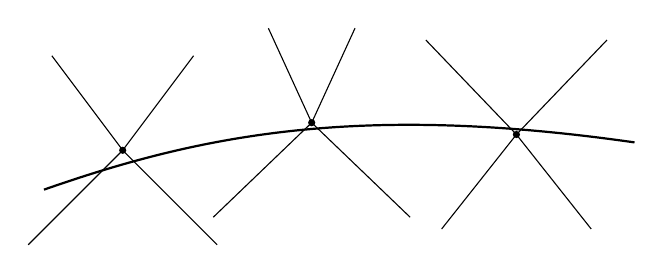
\begin{tikzpicture}[scale=1.0]
\draw[thick] (-4,-0.5) .. controls (-2,0.2) and (0,0.6) .. (3.5,0.1);
\foreach \x/\y/\a/\b in {-3/0/0.9/1.2, -0.6/0.35/0.55/1.25, 2.0/0.2/1.15/0.95} {
  \fill (\x,\y) circle (1.3pt);
  \draw (\x,\y) -- ++(-\a,1.2);
  \draw (\x,\y) -- ++(\a,1.2);
  \draw (\x,\y) -- ++(-\b,-1.2);
  \draw (\x,\y) -- ++(\b,-1.2);
}
\end{tikzpicture}
\caption{A cleaned companion drawing of neighboring local light cones. Their apparent shape changes with coordinates and with the local metric, but the causal classification remains the same.}
\end{figure}

\subsection{Question \& Answer}

A natural question now arises: if the metric has one negative eigenvalue, does that pick out one unique time-like vector?

The answer is no. The invariant statement is about the form, not about a single privileged vector. In a particular inertial coordinate system one may point to the vector \((1,0,0,0)\), but that is a coordinate choice, not a physical absolute. All time-like vectors inside the cone are related to one another by Lorentz transformations. What survives every coordinate change is not one preferred arrow, but the Lorentzian signature itself.

This is also why the shape of the light cone can look different in different coordinates without signaling a real change of physics. One may squash it, tilt it, or otherwise distort its appearance by changing coordinates. The geometry has not changed merely because the drawing has.

\section{Geodesics from Stationary Distance to Stationary Proper Time}

The lecture briefly recalls the older definition of a geodesic before replacing it with something more useful. In standard notation, with dots now denoting derivatives with respect to proper time, the geodesic equation is
\begin{equation}
\ddot x^\mu + \Gamma^\mu{}_{\sigma\rho}\dot x^\sigma \dot x^\rho = 0.
\end{equation}
The spoken sign around the Christoffel term is hesitant, but the standard clean form is the one above.

For actual calculations, however, the variational definition is better. In ordinary space we say that a geodesic is a curve of stationary distance between two points. If the spatial metric is \(g_{mn}\), then
\begin{equation}
ds^2 = g_{mn}\,dx^m dx^n,
\qquad
\int ds = \int \sqrt{g_{mn}\,dx^m dx^n}.
\end{equation}
The geodesic is the curve that makes this integral stationary.

Now the lecture makes its deliberate turn. We are no longer interested in ordinary spatial distance, but in proper time between two space-time events. So we replace the spatial functional by
\begin{equation}
\tau = \int \sqrt{-\,g_{\mu\nu}\,dx^\mu dx^\nu}.
\end{equation}
For a massive particle the corresponding action is defined to be
\begin{equation}
A = -m\tau = -m\int \sqrt{-\,g_{\mu\nu}\,dx^\mu dx^\nu}.
\end{equation}

In the spoken lecture the word ``minimize'' is used repeatedly. The clean statement is slightly subtler. A time-like geodesic makes the proper time stationary and, locally, maximal; because the action carries an explicit minus sign, the same worldline minimizes \(A=-m\tau\). For the mechanics of the problem, the minus sign is exactly what makes the action principle look familiar.

\section{Particle Action, Lagrangian Form, and Euler--Lagrange Equations}

At first sight the proper-time action looks unfamiliar. It is not written as an ordinary integral of ``a function times \(dt\).'' Susskind pauses here for a reason: before we can use the calculus of variations, we must rewrite the action in the conventional form.

We divide the quadratic form inside the square root by \(dt^2\) and compensate by pulling one factor of \(dt\) outside. Then
\begin{align}
A
&= -m\int \sqrt{-\,g_{\mu\nu}(x)\,dx^\mu dx^\nu} \\
&= -m\int \sqrt{-\,g_{\mu\nu}(x)\,\frac{dx^\mu}{dt}\frac{dx^\nu}{dt}}\,dt.
\end{align}
Now the action has the standard form
\begin{equation}
A=\int L\,dt,
\end{equation}
with
\begin{equation}
L=-m\sqrt{-\,g_{\mu\nu}(x)\,\dot x^\mu \dot x^\nu},
\qquad
\dot x^\mu \equiv \frac{dx^\mu}{dt}.
\end{equation}
This is the key practical turn of the lecture: geometry has been translated into mechanics.

\begin{figure}[t]
\centering

\includegraphics[width=0.82\textwidth]{lecture_05_figure_05.png}
\caption{Relativistic particle action rewritten as an integral of the Lagrangian. The board preserves the live transition from the square-root worldline functional to the conventional action form \(A=\int L\,dt\).}
\end{figure}

\begin{figure}[t]
\centering

\includegraphics[width=0.82\textwidth]{lecture_05_figure_06.png}
\caption{The same action a little later, with the Lagrangian isolated more cleanly.}
\end{figure}

Particles move on time-like trajectories, so the quantity under the square root is positive. That matters: the action is only real because for a genuine massive particle the worldline remains inside the light cone.

Once the Lagrangian has been identified, the Euler--Lagrange equations take over:
\begin{equation}
\frac{d}{dt}\left(\frac{\partial L}{\partial \dot x^\mu}\right)=\frac{\partial L}{\partial x^\mu}.
\end{equation}
This is why the variational viewpoint is so useful. The principle of stationary action becomes a differential equation, the relativistic analog of an \(F=ma\)-type law. The geodesic is no longer an abstract curve; it is the motion of a particle determined by a Lagrangian.

\section{Weak-Field Metric and the Newtonian Limit}

Before trusting this formalism in a real gravitational field, the lecture checks it against something familiar. We assume a weak static gravitational field and take, to first order in \(1/c^2\),
\begin{equation}
d\tau^2 = \left(1+\frac{2u(x)}{c^2}\right)dt^2 - \frac{1}{c^2}(dx^2+dy^2+dz^2),
\end{equation}
where \(u(x)\) is the Newtonian gravitational potential.

Plugging this into the action, and restoring the overall factor of \(c^2\) for dimensions, gives
\begin{equation}
A=-mc^2\int \sqrt{1+\frac{2u(x)}{c^2}-\frac{\dot{\mathbf x}^{\,2}}{c^2}}\,dt,
\qquad
\dot{\mathbf x}^{\,2}=\dot x^2+\dot y^2+\dot z^2.
\end{equation}
Now we take the nonrelativistic limit \(c\to\infty\). The point is not to erase every factor of \(1/c^2\), for that would erase the entire correction, but to expand the square root:
\begin{equation}
\sqrt{1+\epsilon}\simeq 1+\frac{\epsilon}{2},
\qquad
\epsilon=\frac{2u-\dot{\mathbf x}^{\,2}}{c^2}.
\end{equation}
Therefore
\begin{align}
L
&= -mc^2\sqrt{1+\frac{2u-\dot{\mathbf x}^{\,2}}{c^2}} \\
&\simeq -mc^2\left(1+\frac{2u-\dot{\mathbf x}^{\,2}}{2c^2}\right) \\
&\simeq -mc^2 - m\,u(x) + \frac{m}{2}\dot{\mathbf x}^{\,2}.
\end{align}
The constant term \(-mc^2\) is irrelevant for the equations of motion, since a constant added to the Lagrangian disappears when we differentiate. What remains is exactly the nonrelativistic Lagrangian \(T-U\):
\begin{equation}
L_{\mathrm{nr}} = \frac{m}{2}\dot{\mathbf x}^{\,2} - m\,u(x).
\end{equation}
Applying the Euler--Lagrange equations now reproduces Newton:
\begin{equation}
m\ddot{\mathbf x} = -m\nabla u.
\end{equation}

This is the major checkpoint of the lecture. The worldline action in curved space-time does not merely resemble mechanics; in the weak-field, slow-motion regime it becomes ordinary mechanics. The immediate lesson is that, to first order,
\begin{equation}
g_{00}\approx 1+\frac{2u}{c^2}.
\end{equation}
For a spherically symmetric source of mass \(M\),
\begin{equation}
u(r)=-\frac{GM}{r},
\end{equation}
and therefore the time-time part of the metric begins to look like
\begin{equation}
g_{00}\approx 1-\frac{2GM}{rc^2}.
\end{equation}

\section{Schwarzschild Metric and the Horizon Puzzle}

We now pass to the real target of the lecture: the metric outside a static, spherically symmetric gravitating body. Because the problem is central, spherical coordinates are the natural coordinates. With the lecture's convention that \(\theta\) is measured from the equator rather than the north pole,
\begin{equation}
d\Omega^2 = d\theta^2 + \cos^2\theta\,d\phi^2,
\end{equation}
and flat three-space becomes
\begin{equation}
dx^2+dy^2+dz^2 = dr^2 + r^2 d\Omega^2.
\end{equation}

From the weak-field result we are led to a first guess:
\begin{equation}
d\tau^2 \approx \left(1-\frac{2GM}{rc^2}\right)dt^2
- \frac{1}{c^2}\left(dr^2+r^2d\Omega^2\right).
\end{equation}
If we introduce the Schwarzschild radius
\begin{equation}
r_s=\frac{2GM}{c^2},
\end{equation}
this becomes
\begin{equation}
d\tau^2 \approx \left(1-\frac{r_s}{r}\right)dt^2
- \frac{1}{c^2}\left(dr^2+r^2d\Omega^2\right).
\end{equation}

This looks promising far from the source, but the lecture deliberately stops here and says that something is terribly wrong. Indeed, when \(r<r_s\), the coefficient of \(dt^2\) changes sign. If we leave the spatial coefficients untouched, then all four diagonal pieces have the same sign. The metric would cease to be Lorentzian; it would no longer have one time-like and three space-like directions.

\subsection{Question \& Answer}

Why must the coefficient of \(dr^2\) change when the coefficient of \(dt^2\) changes sign?

Because the signature must remain Lorentzian everywhere in the domain where the solution is meant to apply. If the \(dt^2\) coefficient flips sign, something else must flip with it. The natural candidate is the radial term. Einstein's equations do not merely suggest this qualitatively; they fix the precise answer:
\begin{equation}
d\tau^2
=
\left(1-\frac{r_s}{r}\right)dt^2
-\frac{1}{c^2\left(1-\frac{r_s}{r}\right)}dr^2
-\frac{r^2}{c^2}d\Omega^2.
\end{equation}
This is the Schwarzschild metric in the form used in the lecture. When \(r\) passes below \(r_s\), both the \(dt^2\) and \(dr^2\) coefficients change sign. The signature remains Lorentzian, but the coordinate roles of \(t\) and \(r\) interchange: \(t\) becomes space-like and \(r\) becomes time-like in these coordinates.

That statement sounds alarming, and the lecture is careful not to pretend otherwise. But it is only a statement about Schwarzschild coordinates. It is not yet a statement that something locally catastrophic happens at the horizon.

To study motion, Susskind then sets \(c=1\) and considers radial infall, so the angular variables are frozen. The Lagrangian becomes
\begin{equation}
L=-m\sqrt{\left(1-\frac{r_s}{r}\right)-\frac{\dot r^2}{1-\frac{r_s}{r}}},
\qquad
\dot r \equiv \frac{dr}{dt}.
\end{equation}
From here one defines the radial momentum and Hamiltonian,
\begin{equation}
p_r=\frac{\partial L}{\partial \dot r},
\qquad
H=p_r\dot r-L.
\end{equation}
A clean reconstruction from the radial Lagrangian gives
\begin{equation}
H
=
\frac{m\left(1-\frac{r_s}{r}\right)}
{\sqrt{\left(1-\frac{r_s}{r}\right)-\frac{\dot r^2}{1-\frac{r_s}{r}}}}.
\end{equation}
Because the Lagrangian has no explicit \(t\)-dependence, \(H\) is conserved. Writing \(H=E\) and solving for \(\dot r\) yields
\begin{equation}
\dot r^2
=
\left(1-\frac{r_s}{r}\right)^2
\left[1-\frac{m^2}{E^2}\left(1-\frac{r_s}{r}\right)\right].
\end{equation}
Near the horizon the bracket tends to \(1\), so
\begin{equation}
\dot r \sim \pm\left(1-\frac{r_s}{r}\right)
\qquad
(r\to r_s).
\end{equation}
Thus, in Schwarzschild coordinate time, the infalling particle slows down and asymptotically freezes at the horizon.

The lecture then notices that there is an easier and cleaner way to see the same freezing effect: look at light rays. For a radial light ray we set \(d\tau^2=0\) and suppress the angular piece. Then
\begin{equation}
\left(1-\frac{r_s}{r}\right)dt^2
-
\frac{1}{1-\frac{r_s}{r}}\,dr^2
=0.
\end{equation}
Multiplying by \(1-r_s/r\) gives
\begin{equation}
\left(1-\frac{r_s}{r}\right)^2dt^2 = dr^2,
\end{equation}
and therefore
\begin{equation}
\frac{dr}{dt}=\pm\left(1-\frac{r_s}{r}\right).
\end{equation}
Even light has Schwarzschild coordinate speed tending to zero as \(r\to r_s\). Nothing can cross the surface in finite external coordinate time \(t\), not even a photon.

\subsection{Question \& Answer}

Why does the horizon take infinite Schwarzschild time to reach but only finite proper time to cross?

Because these are different clocks attached to different descriptions of the same event. The outside observer uses the Schwarzschild coordinate \(t\). The infalling observer uses proper time \(\tau\). Near the horizon,
\begin{equation}
\frac{dr}{dt}\sim -\left(1-\frac{r_s}{r}\right),
\end{equation}
so
\begin{equation}
\frac{dt}{dr}\sim -\,\frac{1}{1-r_s/r}=-\,\frac{r}{r-r_s},
\end{equation}
whose integral diverges logarithmically as \(r\to r_s\). This is the infinite coordinate time.

But nothing singular happens to the local geometry at the horizon. The metric coefficient \(\left(1-r_s/r\right)\) in front of \(dt^2\) goes to zero, so a large coordinate interval \(dt\) can correspond to a small proper interval \(d\tau\). That is why the infalling observer reaches the horizon in finite proper time. The divergence belongs to the coordinate system, not to a physical singularity at \(r=r_s\).

The same point resolves the apparent slowing of light. A radial photon has Schwarzschild coordinate speed \(dr/dt\to 0\), but that is not its local speed measured by an observer falling with it. In a sufficiently small freely falling frame, the metric is locally Minkowskian, and the photon still moves at the speed of light. The horizon is not a place where clocks stop working or photons acquire rest mass. It is a place where Schwarzschild coordinates become awkward.

One further caution from the lecture is worth keeping. The Schwarzschild solution is an exterior solution. For the Earth, \(r_s\) is about a centimeter, far inside the actual matter distribution. There is no Earth horizon. The Schwarzschild geometry is reliable outside the gravitating body; only if the body collapses within its Schwarzschild radius does the horizon become physically relevant.

The lecture ends by leaving one paradox deliberately alive. From the external point of view, matter appears to pile up near the horizon and never quite cross it. How, then, can a black hole grow? The answer is not that it fails to grow, but that the naive coordinate picture is incomplete. That knot is left for later unraveling.

\section{Summary}

The lecture begins in flat space-time because causal language must be secure before curvature can be discussed. From the Minkowski interval we obtain the three causal classes, then the invariant notion of Lorentzian signature, and then the general metric \(g_{\mu\nu}(x)\) with a local light cone at each event. Geodesics are next recast as stationary-action problems, which lets us translate geometry into a particle Lagrangian and derive equations of motion.

That machinery earns its keep in two ways. First, a weak-field metric reproduces Newtonian gravity and identifies \(g_{00}\) with the Newtonian potential to leading order. Second, the same formalism leads to the Schwarzschild metric, where the first naive guess fails on signature grounds and the corrected metric preserves a Lorentzian geometry even across the horizon. In Schwarzschild coordinates both infalling particles and radial light rays freeze as \(r\to r_s\), but the horizon itself is not a physical singularity. The puzzle is therefore not whether anything local breaks there, but how different clocks and different coordinates describe the same crossing.